\chapter{Gravitatie}\label{ch:g9:gravitation}

Een appel laat zijn tak los en valt. De \omterm{def:g2:moon-in-the-sky:moon}{Maan}, boven
dezelfde boomgaard, valt niet. Duizenden jaren lang leken dit twee
losstaande feiten --- tot één geniaal inzicht ze verbond: de
\omterm{def:g2:moon-in-the-sky:moon}{Maan} \emph{is} aan het vallen, eindeloos, om de Aarde heen,
vastgehouden door precies de trek die de appel opeist. Eén wet voor
boomgaard en hemel --- de stoutmoedigste vergelijking die tot die dag
was geschreven, en jouw laatste jaar in dit boek opent ermee.

\section{De universele aantrekking}

\begin{definition}[Gravitatie]\label{def:g9:gravitation:gravitation}
\emph{Gravitatie}\index{gravitatie} is de wederzijdse aantrekking
tussen alle \omterm{def:g3:measuring-mass:mass}{massa}'s: elk stukje materie in het heelal trekt aan elk
ander. Het is de \omterm{def:g2:pushes-and-pulls:force}{kracht} zonder aanraking die je jaren geleden als
``de trek van de Aarde'' ontmoette --- nu onthuld als universeel: de
Aarde trekt aan de appel, de appel trekt aan de Aarde, de
\omterm{def:g2:moon-in-the-sky:moon}{Maan} trekt aan de zeeën, de Zon trekt aan de
planeten, en twee boeken op een plank trekken aan elkaar,
zwakjes, voor altijd.
\end{definition}

\begin{proposition}[De wet van de universele gravitatie]\label{prop:g9:gravitation:law}
Twee lichamen met \omterm{def:g3:measuring-mass:mass}{massa}'s $m_A$ en $m_B$ (in \unit{kg}), waarvan de
middelpunten een afstand $d$ uit elkaar liggen (in \unit{m}),
trekken elkaar aan met even grote, tegengesteld gerichte
\omterm{def:g2:pushes-and-pulls:force}{krachten} langs de verbindingslijn, met grootte
\[
F = G \times \frac{m_A \times m_B}{d^2},
\]
met $F$ in newton (\unit{N}) --- de \omterm{def:g6:measurement-in-science:measuring}{eenheid} van
\omterm{def:g2:pushes-and-pulls:force}{kracht} waarvan het volledige verhaal in het volgende hoofdstuk
begint --- en $G = \qty{6.67e-11}{N.m^2/kg^2}$, de
\emph{gravitatieconstante}, overal in het heelal hetzelfde getal. De
\omterm{def:g2:pushes-and-pulls:force}{kracht} groeit met elke \omterm{def:g3:measuring-mass:mass}{massa} en sterft met het
\emph{kwadraat} van de afstand: twee keer zo ver, vier keer zo zwak;
tien keer zo ver, honderd keer zo zwak.
\end{proposition}

\begin{omfigure}
\begin{tikzpicture}[scale=0.85]
  \draw[thick, fill=omDef, fill opacity=0.4] (1.4,1.4) circle (0.65);
  \node[font=\small] at (1.4,1.4) {$m_A$};
  \draw[thick, fill=omThm, fill opacity=0.4] (8.6,1.4) circle (0.45);
  \node[font=\small] at (8.6,1.4) {$m_B$};
  \draw[-Stealth, very thick, omThm] (2.15,1.4) -- (3.55,1.4);
  \draw[-Stealth, very thick, omDef] (8.05,1.4) -- (6.65,1.4);
  \draw[Stealth-Stealth, omExo] (1.4,0.45) -- (8.6,0.45);
  \node[below, font=\small, omExo] at (5.0,0.35) {$d$};
  \node[above, font=\small] at (5.0,1.75)
    {even grote trek, tegengestelde kant op --- altijd allebei};
\end{tikzpicture}

{\small Universele \omterm{def:g9:gravitation:gravitation}{gravitatie}: twee \omterm{def:g3:measuring-mass:mass}{massa}'s, twee even grote,
tegengestelde trekken langs de verbindingslijn --- de appel trekt
precies zo hard aan de Aarde als de Aarde aan de appel.}
\end{omfigure}

\begin{example}[De wet lezen]\label{ex:g9:gravitation:reading}
Elk kenmerk van de formule spreekt. De \omterm{def:g3:measuring-mass:mass}{massa}'s vermenigvuldigen:
verdubbel een van beide partners en de \omterm{def:g2:pushes-and-pulls:force}{kracht} verdubbelt. De
afstand staat gekwadrateerd in de noemer: de zwaartekracht is een snel
wegstervende fluistering --- de omgekeerd-kwadratische verdunning die je
opnieuw zult tegenkomen bij \omterm{def:g1:light-and-shadows:source}{licht} en \omterm{def:g3:sound-around-us:sound}{geluid}, want het
is de meetkunde van alles wat zich in de ruimte uitspreidt. En de
minuscule grootte van $G$ --- elf nullen achter de komma --- verkondigt
dat \omterm{def:g9:gravitation:gravitation}{gravitatie} het zwakke broertje van de
\omterm{def:g2:pushes-and-pulls:force}{krachten} in de natuur is: ze regeert de kosmos alleen omdat de
\omterm{def:g3:measuring-mass:mass}{massa}'s daarboven monsterlijk zijn en niets haar opheft.
\end{example}

\begin{example}[Waarom boekenplanken niet dichtklappen]\label{ex:g9:gravitation:books}
Twee boeken van \qty{1}{kg}, met de middelpunten \qty{0.1}{m} uit
elkaar:
\[
F = \num{6.67e-11} \times \frac{1 \times 1}{0.1^2}
= \qty{6.67e-9}{N}
\]
--- een paar miljardsten van een newton, het \omterm{def:g4:weight-and-mass:weight}{gewicht} van het
stofje van een stofje. Nu de Aarde en de appel: vervang één boek door
\qty{5.97e24}{kg} \omterm{def:g4:solar-system:planet}{planeet} en de afstand door haar straal van
\qty{6.4e6}{m}, en dezelfde wet levert de vertrouwde ruk van een middag
in de boomgaard. Universeel betekent universeel --- alleen de \omterm{def:g3:measuring-mass:mass}{massa}'s
bepalen wie het merkt.
\end{example}

\section{De vallende Maan}

\begin{example}[Het kanon op de berg]\label{ex:g9:gravitation:cannon}
Het gedachte-experiment van het inzicht zelf. Vuur een kanonskogel
horizontaal af vanaf een hoge top: hij beschrijft een boog en landt.
Vuur hem sneller af: hij landt verder --- terwijl de trek van de Aarde
zijn \omterm{def:g6:describing-motion:trajectory}{baan} de hele tijd krombuigt. Stel je nu voor dat je hem zo snel
afvuurt dat het oppervlak van de ronde Aarde, terwijl hij valt,
\emph{er met dezelfde \omterm{def:g7:motion-average-speed:formula}{snelheid} onderuit krult}: de kogel valt eindeloos
en landt nooit --- hij cirkelt om de \omterm{def:g4:solar-system:planet}{planeet}. Dat eeuwige vallen
heeft een vertrouwde naam: een \emph{\omterm{def:g6:sun-earth-moon:axisorbit}{omloopbaan}}. Niets houdt
een rondgaand lichaam ``omhoog''; het valt met stijl.
\end{example}

\begin{omfigure}
\begin{tikzpicture}[scale=0.85]
  % the curving Earth: only the upper limb of a much larger circle
  \fill[omDef, opacity=0.25] (-1.01,0.23) arc (106:74:20)
    -- (10.01,-0.9) -- (-1.01,-0.9) -- cycle;
  \draw[thick] (-1.01,0.23) arc (106:74:20);
  % the mountain and its gun
  \draw[thick, fill=omExo!30]
    (-1.1,0.2) -- (0.25,2.3) -- (1.3,0.72) -- cycle;
  \draw[thick, fill=omExo!60] (0.0,2.18) rectangle (0.55,2.42);
  \node[left, font=\small] at (-0.85,2.3) {het bergkanon};
  % three shots, each faster than the last
  \draw[omThm, thick] (0.55,2.32)
    .. controls (1.6,2.25) .. (2.4,0.9);
  \draw[omThm, thick] (0.55,2.35)
    .. controls (2.8,2.25) .. (4.9,1.0);
  \draw[omThm, thick] (0.55,2.38)
    .. controls (4.2,2.35) .. (7.5,0.8);
  \node[right, font=\small, omThm] at (1.9,3.0)
    {sneller: verder};
  % fast enough: the fall closes into an orbit
  \draw[omMeth, very thick, dashed] (0.3,2.35) arc (101:73:21.76);
  \node[right, font=\small, omMeth] at (6.4,3.35)
    {snel genoeg: het vallen wordt een baan};
\end{tikzpicture}

{\small Het bergkanon: elk sneller schot valt verder om de krommende
Aarde heen --- tot vallen en krommen bij elkaar passen en de
kanonskogel een \omterm{def:g6:describing-motion:trajectory}{baan} beschrijft.}
\end{omfigure}

\begin{proposition}[Wat gravitatie aandrijft]\label{prop:g9:gravitation:runs}
Eén wet, de hele hemel: de \omterm{def:g2:moon-in-the-sky:moon}{Maan} is de eeuwige kanonskogel van
de Aarde, die één keer per maand om ons heen valt; de
planeten vallen net zo om de Zon heen --- de dichterbij staande
sneller, zoals het omgekeerde kwadraat eist; kometen duiken uit het
donker naar binnen in lange vallende lussen; en elke kunstmatige
satelliet --- weerogen, navigatiebakens, het bemande station dat elke
negentig minuten rondgaat --- rijdt op de wiskunde van het bergkanon.
Niets aan de hemel is opgehangen. Alles valt, en mist.
\end{proposition}

\begin{example}[Getijden: de Maan trekt terug]\label{ex:g9:gravitation:tides}
De wederkerigheid heeft een handtekening die in water is geschreven. De
trek van de \omterm{def:g2:moon-in-the-sky:moon}{Maan} aan de Aarde is het sterkst op de oceaan die
naar haar toe gekeerd is en het zwakst aan de verre kant --- dus stapelt
de zee zich zachtjes tegelijk naar de \omterm{def:g2:moon-in-the-sky:moon}{Maan} toe en ervandaan op,
en terwijl de Aarde onder die bulten door draait, zien kusten het water
rijzen en dalen: de \emph{getijden}, op de meeste dagen twee keer. De
Zon steekt haar hand toe --- op één lijn bij nieuwe en
\omterm{ex:g2:moon-in-the-sky:shapes}{volle maan} voor het grote springtij. Vissers lezen de
\omterm{def:g2:moon-in-the-sky:moon}{Maan} al millennia; de wet leest haar terug.
\end{example}

\begin{remark}[Wat de wet niet zegt]\label{rem:g9:gravitation:notsay}
De grote vergelijking berekent de \omterm{def:g2:pushes-and-pulls:force}{kracht} tot in verfijnde
nauwkeurigheid en verklaart geen greintje van \emph{hoe} twee lichamen
elkaar over lege leegte beetpakken --- de auteur ervan noemde die vraag
zelf open en liet haar, schitterend, onbeantwoord. Diepere antwoorden
bestaan --- de universitaire jaren van deze cursus bereiken het moderne,
waarin \omterm{def:g3:measuring-mass:mass}{massa} de meetkunde kromt waarin ze zelf woont --- maar elke
eerlijke natuurkundige sindsdien heeft de les herhaald die je van deze
bladzijde mag meenemen: een wet kan volmaakt bruikbaar zijn, volmaakt
getoetst, en toch haar laatste geheim bewaren.
\end{remark}

\begin{omfigure}
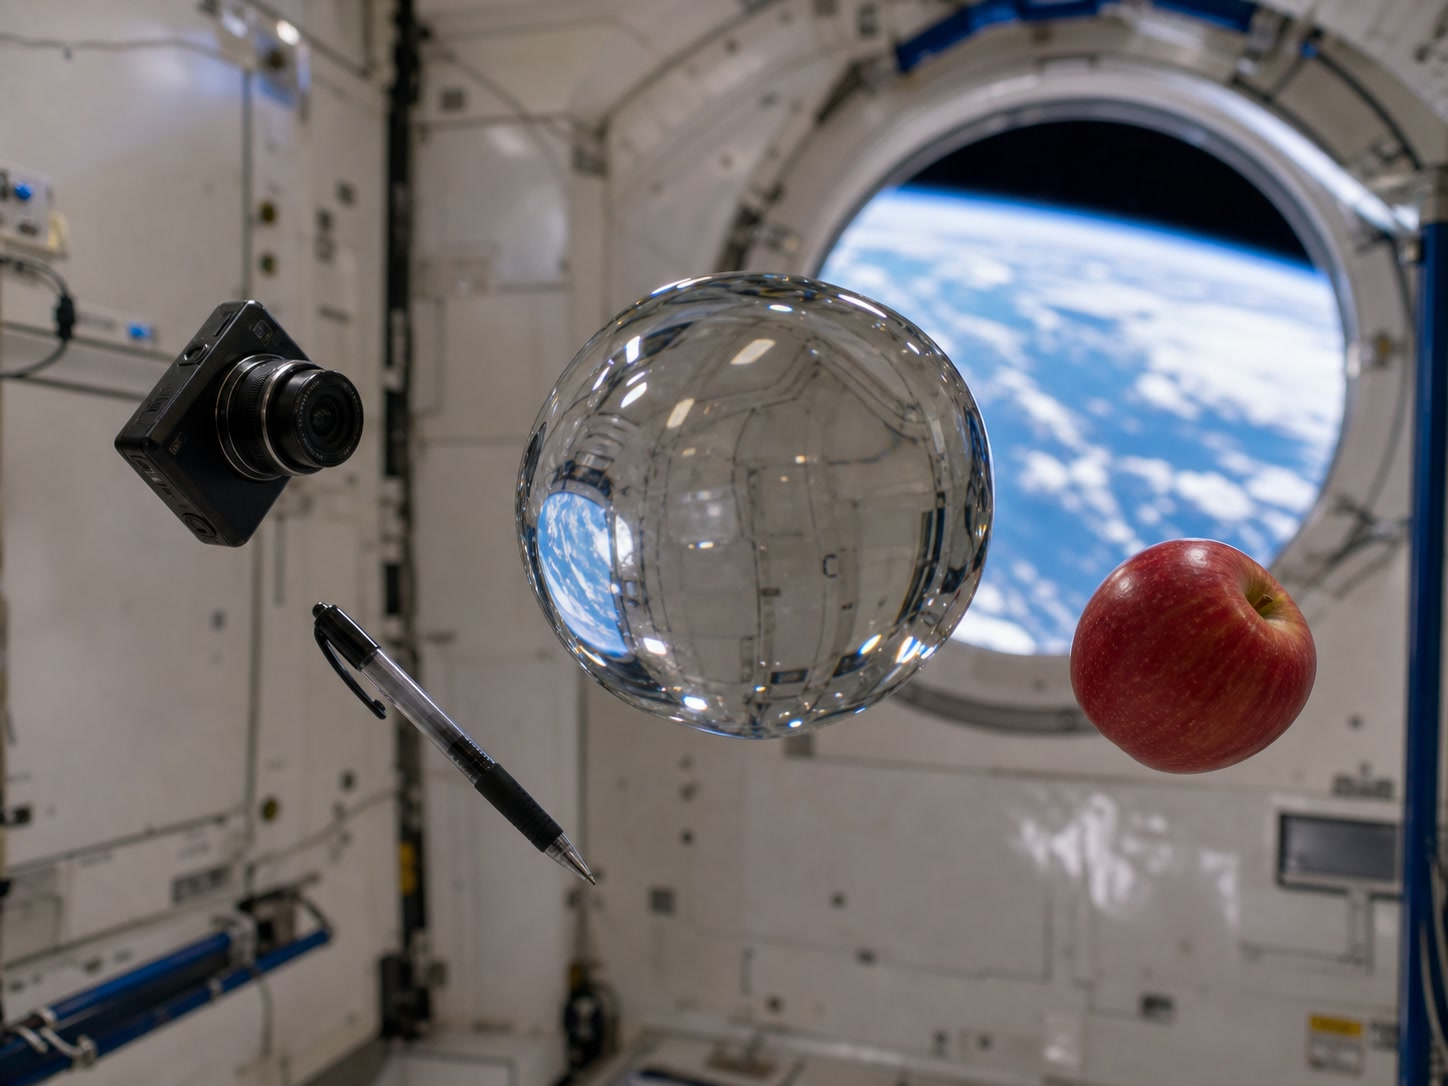
\includegraphics[width=0.5\linewidth]{images/book1/ai/g9-gravitation-weightless.jpg}

{\small Vrije val, dagelijks beleefd: het ruimtestation en alles erin vallen samen om de Aarde heen, zodat niets ergens op drukt --- camera's, pennen, appels en water zweven.}
\end{omfigure}

\section{Oefeningen}

\begin{exercise}[$\star$]\label{exo:g9:gravitation:1}
Formuleer de wet van de universele \omterm{def:g9:gravitation:gravitation}{gravitatie} --- formule,
eenheden, en de twee kenmerken (\omterm{def:g3:measuring-mass:mass}{massa}'s, afstand) in woorden.
\end{exercise}

\begin{exercise}[$\star$]\label{exo:g9:gravitation:2}
De Aarde trekt met \qty{1}{N} aan de appel. Met welke
\omterm{def:g2:pushes-and-pulls:force}{kracht} trekt de appel aan de Aarde? Waarom versnelt er maar
één van de twee zichtbaar?
\end{exercise}

\begin{exercise}[$\star$]\label{exo:g9:gravitation:3}
Twee satellieten draaien hun \omterm{def:g6:describing-motion:trajectory}{baan} op afstanden $d$ en $2d$
vanaf het middelpunt van de Aarde. Vergelijk de
gravitatiekrachten op hen (gelijke \omterm{def:g3:measuring-mass:mass}{massa}'s). En op $10 d$?
\end{exercise}

\begin{exercise}[$\star$]\label{exo:g9:gravitation:4}
Bereken de aantrekking tussen twee danspartners van \qty{80}{kg} op
\qty{0.5}{m} afstand --- en geef commentaar op romantiek tegenover
\omterm{def:g9:gravitation:gravitation}{gravitatie}.
\end{exercise}

\begin{exercise}[$\star$]\label{exo:g9:gravitation:5}
Welke twee snelheden komen in het verhaal van het bergkanon precies
overeen voor het rondgaande schot? Wat is een \omterm{def:g6:describing-motion:trajectory}{baan}, in drie
woorden?
\end{exercise}

\begin{exercise}[$\star$]\label{exo:g9:gravitation:6}
``De astronauten zweven omdat er daarboven geen zwaartekracht
is.'' Sloop deze bewering met de kanonskogel: wat doen het station en de
bemanning allebei?
\end{exercise}

\begin{exercise}[$\star$]\label{exo:g9:gravitation:7}
Waarom regeert \omterm{def:g9:gravitation:gravitation}{gravitatie}, het zwakke broertje van de natuur,
toch de kosmos? Twee redenen uit het hoofdstuk.
\end{exercise}

\begin{exercise}[$\star$]\label{exo:g9:gravitation:8}
Waar komen de getijden vandaan, en waarom op de meeste dagen twee keer?
Wanneer slaan de grootste toe?
\end{exercise}

\begin{exercise}[$\star\star$]\label{exo:g9:gravitation:9}
De \omterm{def:g2:moon-in-the-sky:moon}{Maan} (\qty{7.3e22}{kg}) draait haar \omterm{def:g6:describing-motion:trajectory}{baan} op
\qty{3.8e8}{m} van de Aarde (\qty{5.97e24}{kg}). Bereken hun
aantrekking, van begin tot eind in wetenschappelijke notatie --- en
bewonder hoeveel cijfers de macht van tien in het antwoord draagt.
\end{exercise}

\begin{exercise}[$\star\star$]\label{exo:g9:gravitation:10}
Op het oppervlak van de \omterm{def:g2:moon-in-the-sky:moon}{Maan} kromp je \omterm{def:g4:weight-and-mass:weight}{gewicht}
tot een zesde (denk aan de stuiterende astronauten). Leg met de twee
knoppen van de wet --- de kleinere \omterm{def:g3:measuring-mass:mass}{massa} van de
\omterm{def:g2:moon-in-the-sky:moon}{Maan}, haar kleinere straal --- uit hoe een zesde kan ontstaan
bij een lichaam dat tachtig keer lichter is dan de Aarde.
\end{exercise}

\begin{exercise}[$\star\star$]\label{exo:g9:gravitation:11}
Mercurius rondt de Zon in $88$ dagen, Neptunus in $165$ jaar. Lees dit
patroon af uit het omgekeerde kwadraat: wat doet het wegsterven van de
zwaartekracht met de afstand met de greep van de Zon, en dus met het
tempo van de buitenste familie?
\end{exercise}

\begin{exercise}[$\star\star\star$]\label{exo:g9:gravitation:12}
Een geostationaire satelliet hangt schijnbaar bewegingloos boven één
punt van de evenaar --- de schotelantennes bewegen nooit. Breng die
schijn in overeenstemming met \cref{prop:g9:gravitation:runs}: hoe groot
moet zijn omlooptijd zijn, welke kant op moet hij cirkelen, en waarom
betekent ``hangen'' hier ``in volmaakte pas met de draaiende Aarde
vallen''?
\end{exercise}

\section{Probleem: de erfenis van de kanonskogel}

\begin{problem}[{Weekendprobleem --- van de boomgaard naar de baan; de
appel, het kanon en de Maan doorgelicht met één wet; het
lanceringsbord}]\label{pb:g9:gravitation:1}
Een avond aan de voorlichtingsbalie van het ruimteagentschap: één wet,
$G = \qty{6.67e-11}{N.m^2/kg^2}$, \omterm{def:g3:measuring-mass:mass}{massa} van de Aarde
\qty{5.97e24}{kg}, straal van de Aarde \qty{6.4e6}{m}.

\medskip\noindent\textbf{Deel I --- De doorlichting van de appel.}
\begin{enumerate}
  \item Bereken de trek van de Aarde aan een appel van \qty{0.1}{kg}
        aan het oppervlak (middelpunten gescheiden door één
        aardstraal).
  \item Met welke \omterm{def:g2:pushes-and-pulls:force}{kracht} trekt de appel terug aan de Aarde?
        Noem het woord van de wet voor deze tweezijdige boekhouding.
  \item Til de appel op tot twee aardstralen van het middelpunt. Wat
        wordt er van de trek?
  \item Een bezoeker vraagt waarom de formule de afstand tot het
        \emph{middelpunt} van de Aarde gebruikt en niet die tot de
        grond. Geef het eerlijke korte antwoord (de hele
        \omterm{def:g4:solar-system:planet}{planeet} trekt, en haar verspreide trekken tellen op alsof
        ze uit het middelpunt komen --- een stelling waar de grote
        auteur zelf jaren over deed om haar te bewijzen).
\end{enumerate}

\medskip\noindent\textbf{Deel II --- Het lanceringsbord.}
\begin{enumerate}[resume]
  \item De satelliet van vandaag weegt \qty{2000}{kg}. Zijn
        \omterm{def:g4:weight-and-mass:weight}{gewicht} aan het oppervlak, volgens de wet? (Of volgens de
        snelweg die het volgende hoofdstuk benoemt: ongeveer
        \qty{9.8}{N} per \omterm{def:g3:measuring-mass:units}{kilogram}.)
  \item In zijn werkbaan op \qty{1.28e7}{m} van het
        middelpunt --- twee aardstralen --- welk deel van zijn
        oppervlaktegewicht oefent de zwaartekracht dan nog op
        hem uit?
  \item ``Dus daarboven is er nog echte zwaartekracht?'' Bevestig het
        met het getal --- en leg uit wat de satelliet met die trek doet
        in plaats van neer te storten.
  \item Het lanceringscommentaar zegt: ``de baansnelheid moet
        bij de val passen''. Vertel het verhaal van het bergkanon in
        twee zinnen na voor de brochure van de bezoekers.
\end{enumerate}

\medskip\noindent\textbf{Deel III --- Het grootboek van de
\omterm{def:g2:moon-in-the-sky:moon}{Maan}.}
\begin{enumerate}[resume]
  \item Met de \omterm{def:g2:moon-in-the-sky:moon}{Maan} op \qty{3.8e8}{m}: op hoeveel aardstralen
        rijdt ze? (Eén decimaal.)
  \item Volgens het omgekeerde kwadraat is de zwaartekracht daar
        vervaagd tot ruwweg welk deel van haar sterkte aan het
        oppervlak? (Kwadrateer je vorige antwoord.)
  \item Het grote inzicht, opnieuw verteld: de appel in de boomgaard
        valt in zijn eerste \omterm{def:g2:measuring-time:second}{seconde} ongeveer vijf \omterm{def:g2:measuring-length:units}{meter}; de
        \omterm{def:g2:moon-in-the-sky:moon}{Maan} ``valt'' elke \omterm{def:g2:measuring-time:second}{seconde} nauwelijks een millimeter naar
        de Aarde toe --- en komt toch nooit aan. Verbind de twee feiten
        via je antwoorden 9 en 10: waarom is de val van de
        \omterm{def:g2:moon-in-the-sky:moon}{Maan} duizenden keren zachter, en waarom eindeloos?
  \item Sluit de voorlichtingsavond af: één wet, drie uitvoerenden ---
        appel, satelliet, \omterm{def:g2:moon-in-the-sky:moon}{Maan}. Schrijf de slotzin van het bord
        die hen verenigt.
\end{enumerate}
\end{problem}
